\chapter{Machine learning}
\label{cap:teoria}
\intro{Per comprendere al meglio gli argomenti trattati nel capitolo successivo è necessaria un'introduzione teorica} \\
Il machine learning è un'applicazione della statistica che si concentra sullo sviluppo di algoritmi in grado di imparare dai dati che vengono loro forniti in input.
Da un punto di vista più filosofico il machine learning è interessante perché sviluppando la nostra conoscenza su di esso stiamo di conseguenza migliorando la nostra comprensione dei principi su cui si sorregge l'intelligenza \footcite[p.~97]{Goodfellow-et-al-2016}.
Gli algoritmi di machine learning si suddividono in due categorie principali:

\begin{itemize}
    \item apprendimento supervisionato: gli algoritmi che appartengono a questa categoria apprendono quali risultati generare seguendo la guida di un set di dati etichettati e con un output predefinito\footcite{site:machine-learning}.

    \item apprendimento non supervisionato: gli algoritmi non supervisionati, anche conosciuti come apprendimento automatico, analizzano e raggruppano dataset non etichettati. Questi algoritmi riconoscono raggruppamenti di dati (cluster) senza la necessità dell'intervento umano\footcite{site:machine-learning}.
\end{itemize}

Tali algoritmi vengono utilizzati nel progetto per il processo di classificazione. \\
La classificazione è un metodo che consente di prevedere a quale classe un determinato input appartenga. 
Quindi generalizzando un'entità viene rappresentata come vettore in uno spazio delle feature, tipicamente \( R^n \), successivamente vengono eseguite delle operazioni sul vettore che producono un valore preso da un insieme di etichette L noto a priori, il classificatore è quindi una funzione \( R^n \rightarrow L \). \\
Un classico esempio di classificazione è fornito dal dataset Iris\footcite{site:iris-dataset}, è uno dei primi dataset utilizzati in letteratura per sperimentare i metodi di classificazione; contiene 3 classi composte da 50 istanze ciascuna, ogni classe si riferisce a un tipologia differente di iris (Fig.~\ref{fig:iris-images}).

\begin{figure}[!h] 
    \centering 
    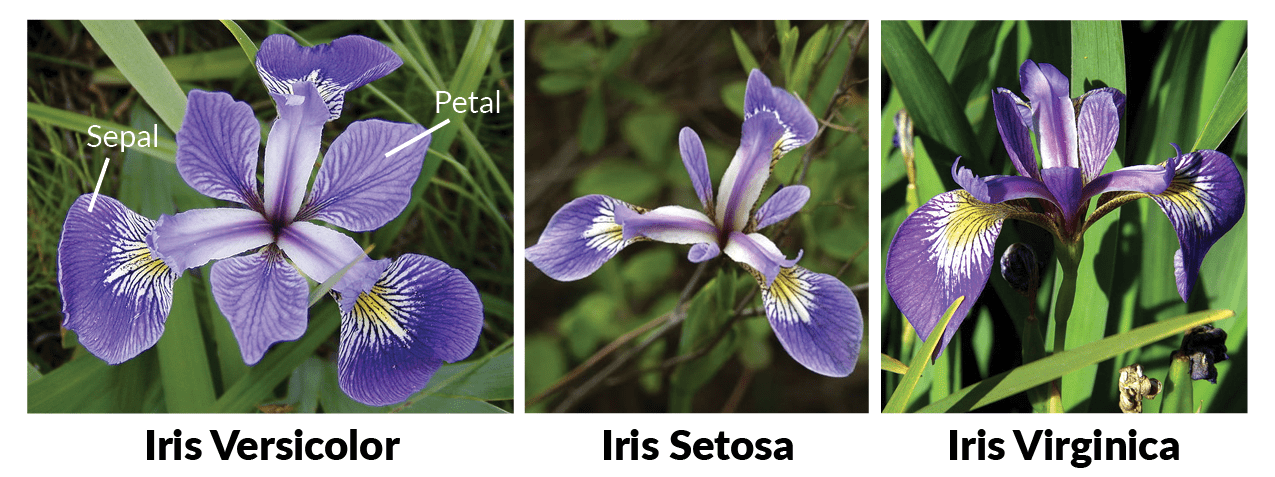
\includegraphics[width=0.8\columnwidth]{teoria/iris-images.png} 
    \caption{Tre tipologie di pianta}
    \label{fig:iris-images}
  \end{figure}

In fase di addestramento vengono utilizzate le feature e le etichette (Fig.~\ref{fig:iris-schema}) di ciascuna pianta e in fase di test l'algoritmo utilizza le caratteristiche apprese per eseguire una classificazione su dati che non ha ricevuto durante il training.

\begin{figure}[!h] 
    \centering 
    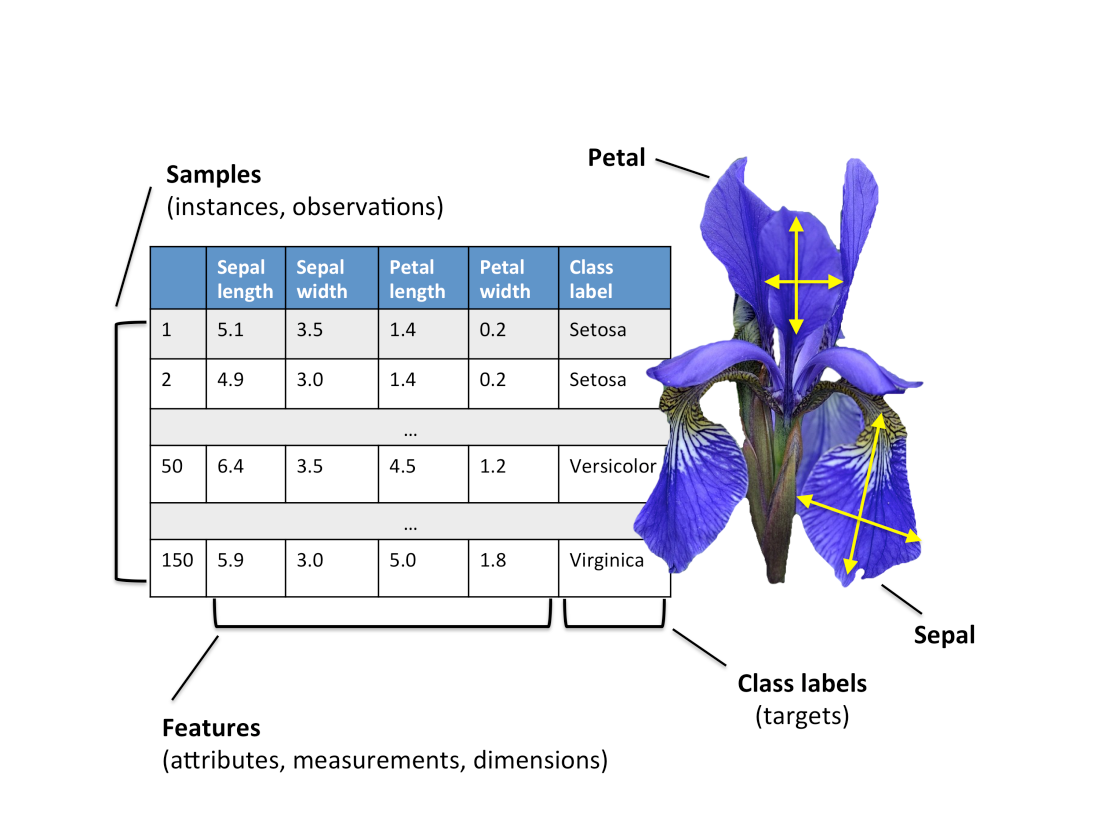
\includegraphics[width=0.8\columnwidth]{teoria/iris-schema.png} 
    \caption{Schema delle feature}
    \label{fig:iris-schema}
  \end{figure}

L'introduzione al machine learning è utile per presentare le applicazioni di tale disciplina utilizzate ai fini del progetto:
\begin{itemize}
    \item Clustering
    \item PCA
    \item Reti neurali
    \item Deep learning
    \item Autoencoder
\end{itemize}
Gli elementi citati in precedenza vengono introdotti e trattati nelle sezioni seguenti.

\section{K-means}
Il K-means è un algoritmo non supervisionato che viene utilizzato per il clustering, ossia per la suddivisione del dataset in gruppi che contengono caratteristiche simili.
Suddivide un set di dati in gruppi simili sulla base della distanza tra i loro centroidi. 
Il centroide, è la media di tutti i punti presenti all'interno del cluster.

Il numero K sta a indicare quanti cluster dovranno essere assegnati dall'algoritmo, più il numero di cluster è elevato più essi saranno piccoli e dettagliati al contrario se i cluster sono pochi il risultato saranno dei cluster più grandi ma meno dettagliati.

Ad esempio se volessimo clusterizzare un insieme di animali composto da mammiferi e uccelli utilizzando K=2 l'algoritmo creerebbe due cluster uno contenente i mammiferi e uno gli uccelli (cluster grandi e poco dettagliati).
Se aumentassimo il numero di cluster l'algoritmo sarebbe in grado di essere più specifico andando a creare una quantità molto più elevata di cluster ben dettagliati contenenti meno elementi.
Quindi è importante scegliere con cura il numero iniziale K da assegnare, per semplificare questa operazione esistono dei metodi di supporto:
\begin{itemize}
    \item Il metodo del gomito sfrutta l’inerzia, ossia la somma delle distanze al quadrato dei punti dal centroide (SSE, Sum of Squared Errors). Con l'aumento dei cluster, l’inerzia diminuisce, ma dopo un certo punto, la riduzione diventa superflua, venendo a creare una curva a gomito. Il punto in cui la curva si piega indica il numero di cluster da utilizzare.
    
    \begin{figure}[!h] 
        \centering 
        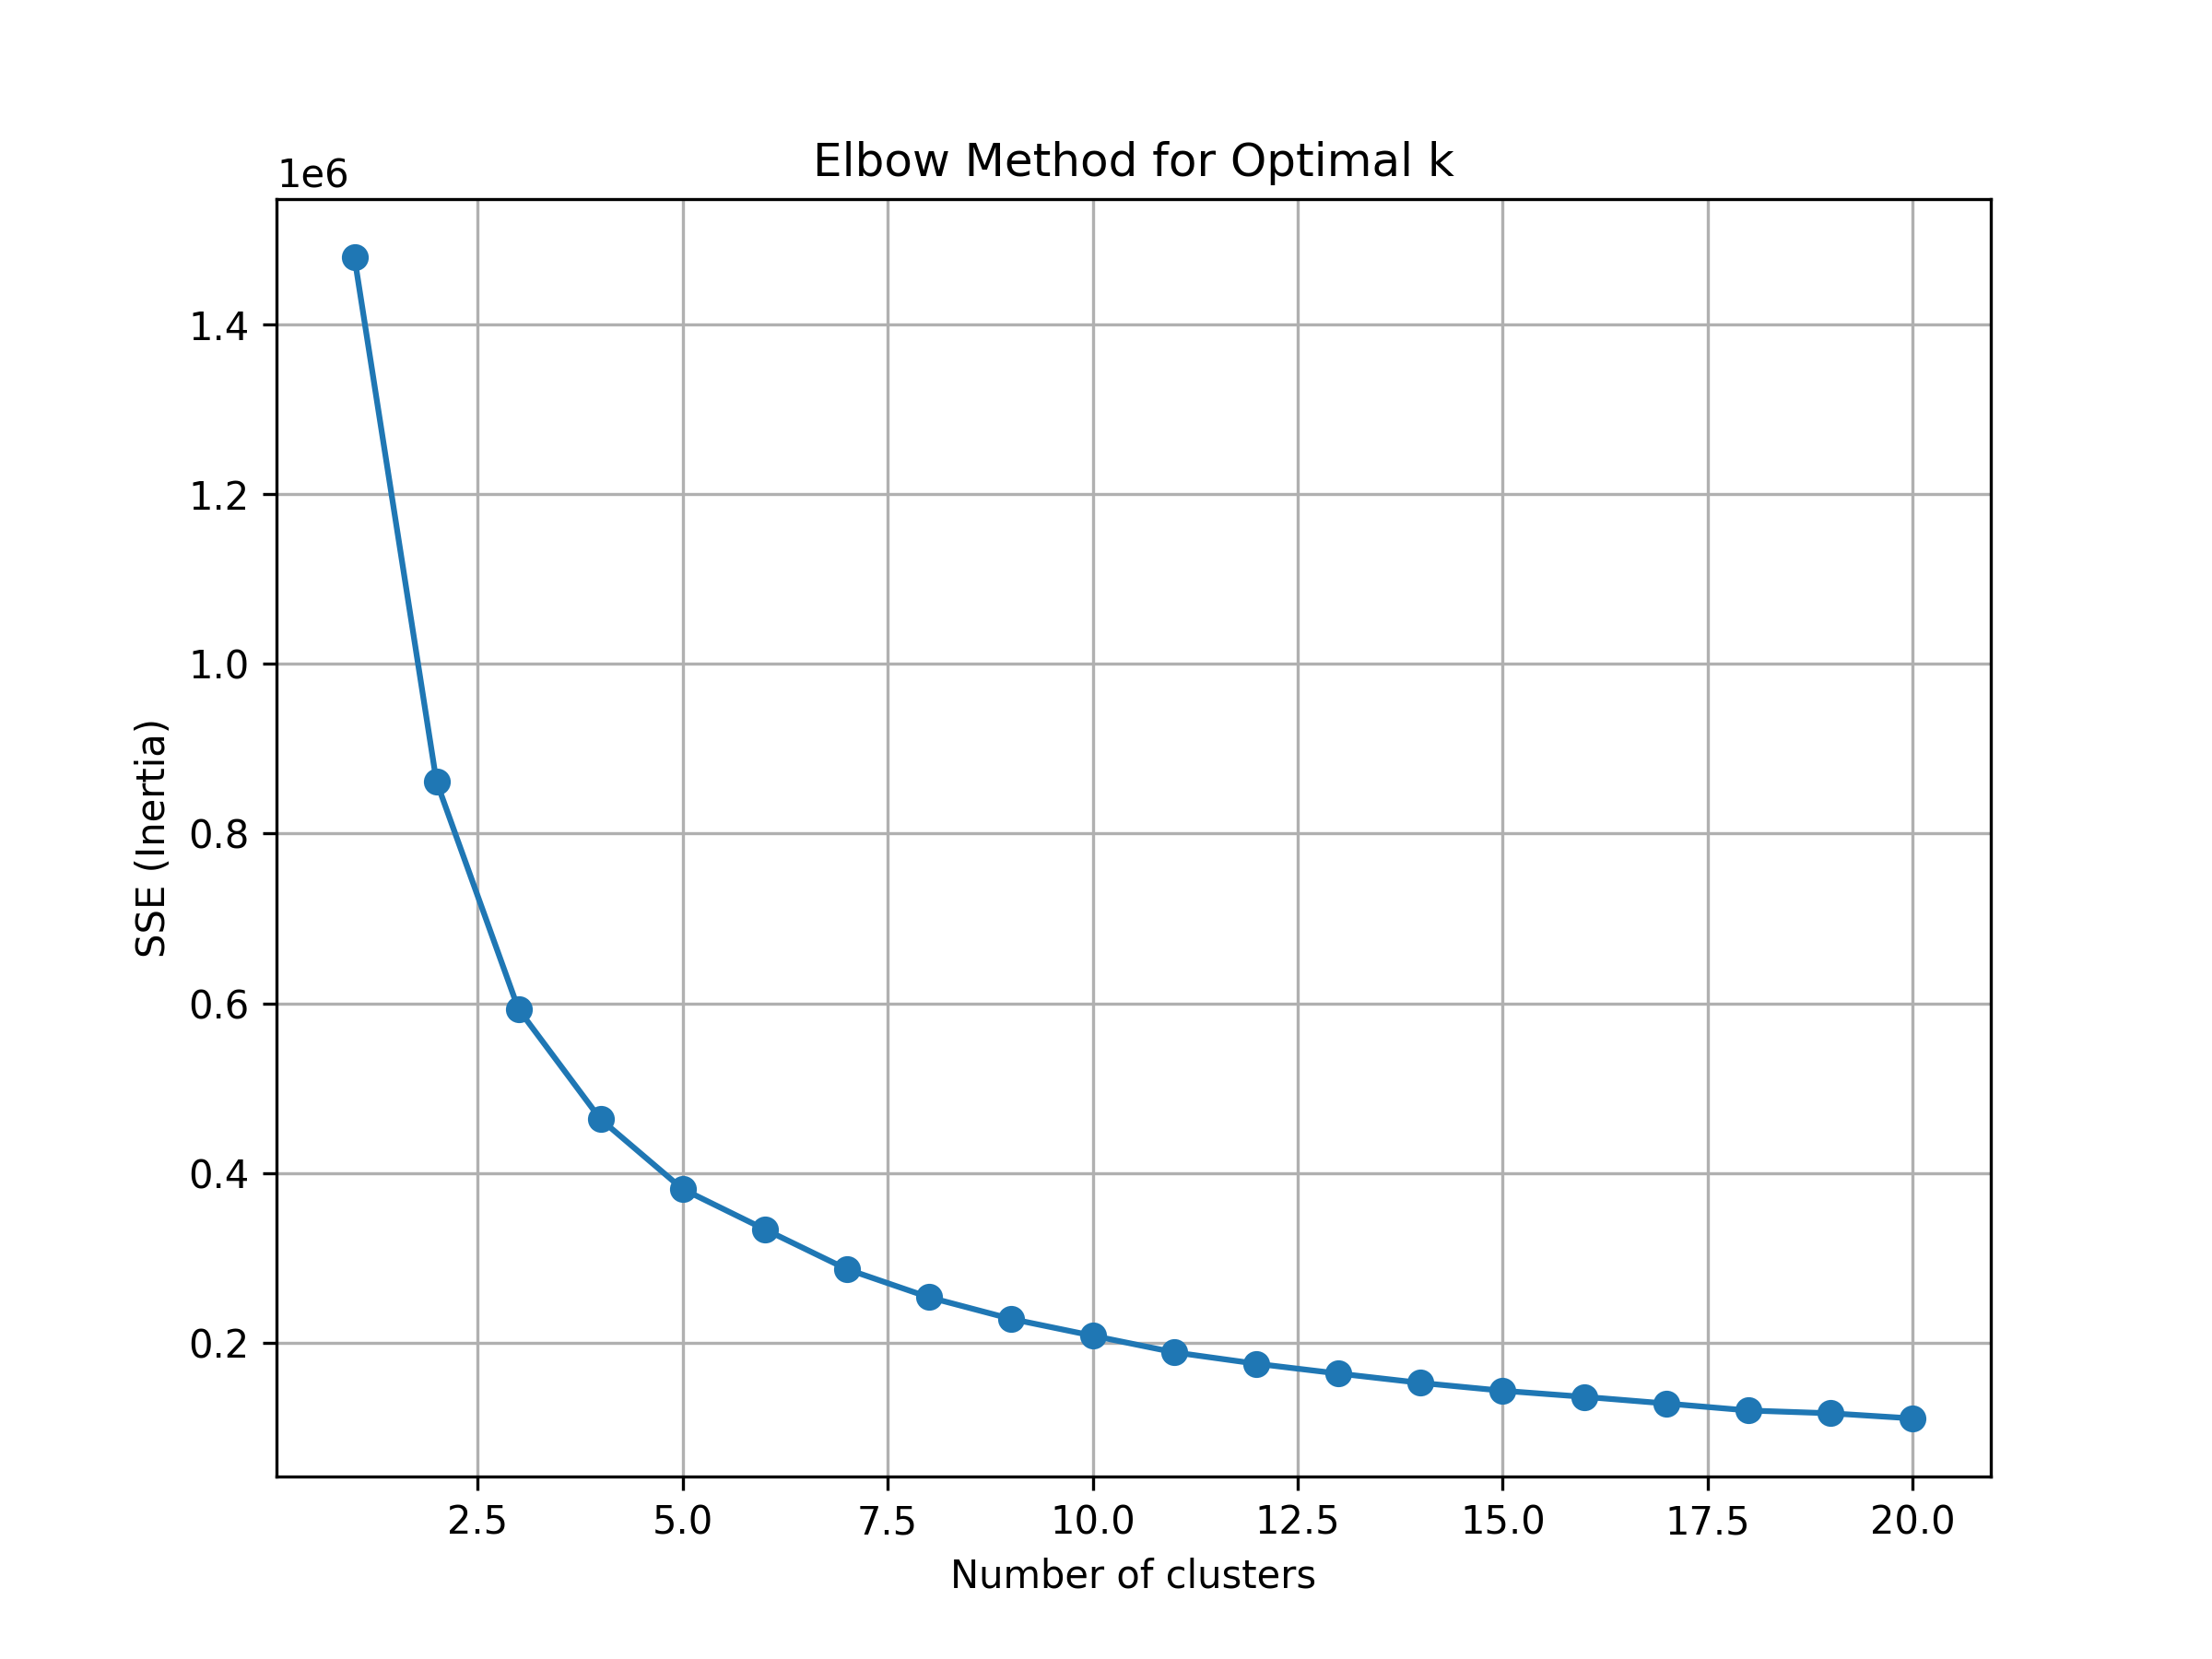
\includegraphics[width=0.7\columnwidth]{teoria/elbow_method.png} 
        \caption{Grafico rappresentante il metodo del gomito}
        \label{fig:gomito}
      \end{figure}

    \item Il Silhouette Score indica quanto i punti appartenenti a un cluster sono simili tra loro e quanto differiscono dai punti contenuti negli altri cluster.
    Varia tra -1 e 1, se il valore è vicino a 1 il punto è all'interno del suo cluster e ben separato dai cluster limitrofi, se è vicino a 0 il punto è confinante tra due cluster infine un valore negativo indica l'assegnazione a un cluster sbagliato.
\end{itemize}

\section{PCA}
L'analisi dei componenti principali è un algoritmo non supervisionato in grado di estrarre le informazioni più rilevanti da dataset di grandi dimensioni, riducendo così la complessità del modello ed evitando che si presenti il fenomeno della "maledizione della dimensionalità"\footcite{site:PCA}.

La maledizione della dimensionalità si verifica all'aumentare della dimensionalità dei dati: con l'aumentare delle dimensioni, il volume dello spazio aumenta in maniera esponenziale, rendendo difficile l'elaborazione da parte degli algoritmi di machine learning, che dovranno lavorare su dati molto sparsi con conseguenze negative per le prestazioni.

Tra gli ulteriori vantaggi che hanno portato all'adozione della PCA sono presenti la riduzione dei tempi di calcolo dovuta alla minor quantità di feature e la possibilità di visualizzare i risultati del clustering su un grafico cartesiano bidimensionale (Fig.~\ref{fig:pca-chart}) aumentando il livello di comprensione dell'utente.

\begin{figure}[!h] 
    \centering 
    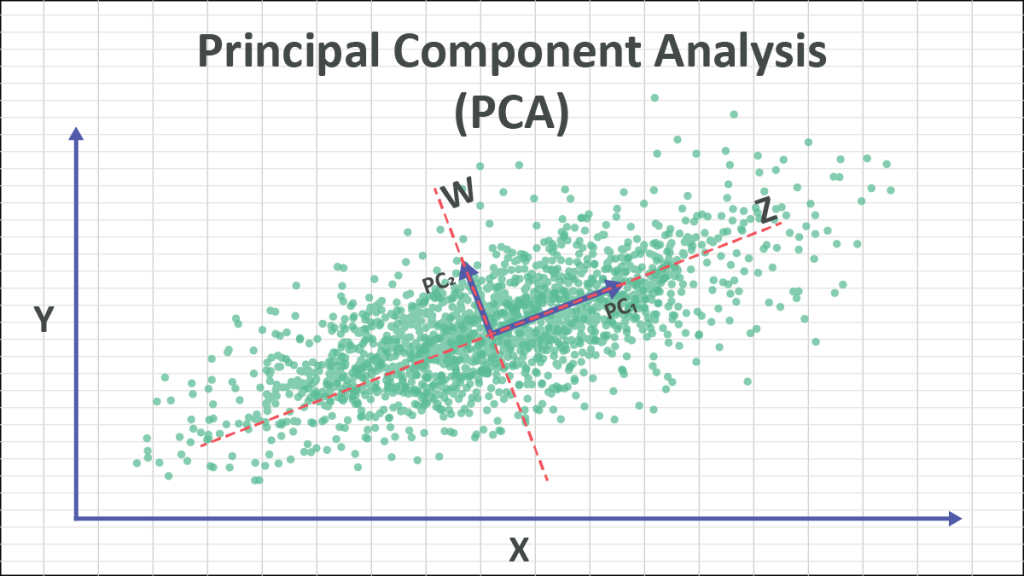
\includegraphics[width=0.7\columnwidth]{teoria/pca-chart.png} 
    \caption{Grafico contenente PCA}
    \label{fig:pca-chart}
  \end{figure}

\section{Reti neurali}
Le reti neurali (Fig.~\ref{fig:rete-neurale}) sono un processo di machine learning che sfrutta nodi interconnessi tra di loro (anche chiamati neuroni) in una struttura a strati ispirata al cervello umano (da qui neural network).
In genere consistono di un sistema adattivo utilizzato dai computer per imparare dagli errori commessi e automigliorarsi\footcite{site:rete-neurale}.

\begin{figure}[!h] 
    \centering 
    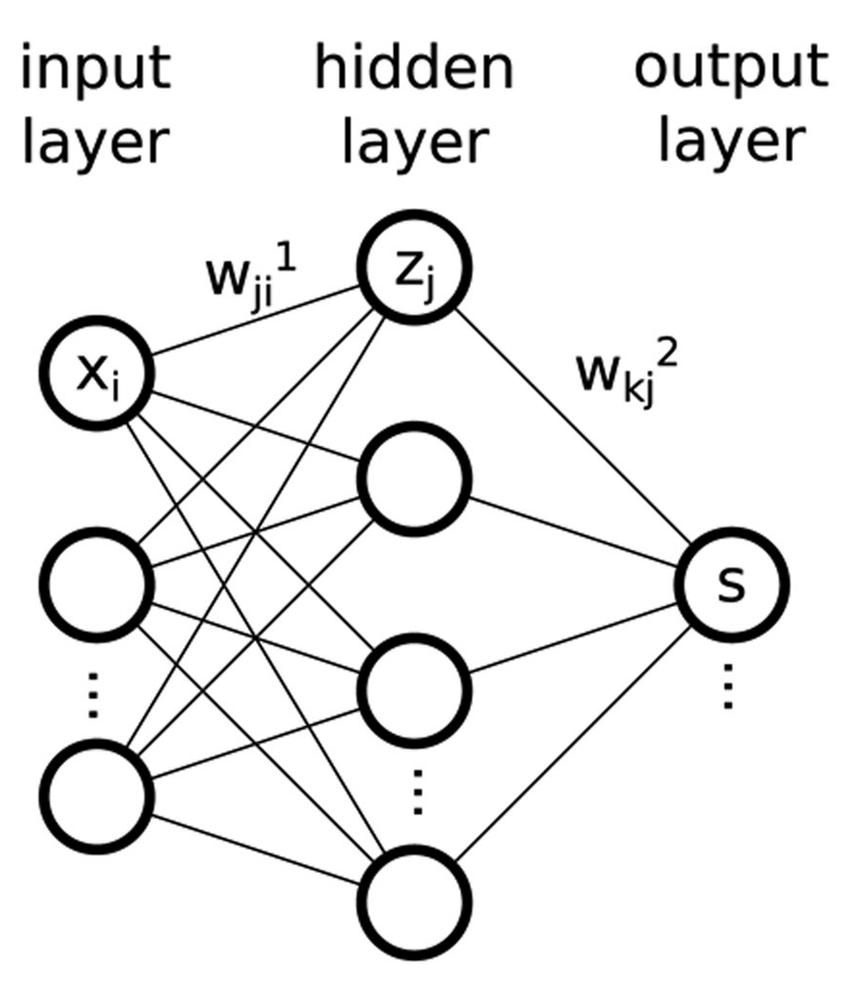
\includegraphics[width=0.4\columnwidth]{teoria/reteneurale.png} 
    \caption{Esempio di rete neurale}
    \label{fig:rete-neurale}
  \end{figure}

\subsubsection{Struttura}
All'interno di una rete neurale sono presenti:
\begin{itemize}
    \item Input layer: riceve l'input che la rete deve elaborare.
    \item Hidden layer: possono essere uno o più e si occupano della elaborazione del dato in input.
    \item Output layer: mostra l'output dell'elaborazione.
\end{itemize}

\subsection{Apprendimento}
Gli strati densi (dense layers) sono alla base della rete neurale e sono composti dai neuroni.
Ogni layer è interconnesso con lo strato che lo precede e con quello successivo, in particolare ogni neurone dello strato è connesso a ogni neurone dello strato successivo.

\subsubsection{Funzionamento del neurone}

\begin{itemize}
    \item Ogni connessione ha un peso che indica la forza della connessione e il suo valore può essere positivo o negativo.
    \item L'input che un neurone riceve da ciascuno dei neuroni a cui è connesso si calcola moltiplicando il segnale proveniente da quel neurone per il peso sulla connessione.
    \item L'input totale del neurone è la sommatoria delle attivazioni che il neurone riceve dagli altri neuroni.
    \item Lo stato di attivazione finale viene calcolato attraverso una funzione di attivazione (ad esempio RELU o sigmoide, Fig.~\ref{fig:relu-sigmoid}).
    \item L'output dei neuroni viene inviato ai neuroni successivi.
\end{itemize}
Lo schema successivo mostra il procedimento appena descritto (Fig.~\ref{fig:neurone})

\begin{figure}[!h] 
    \centering 
    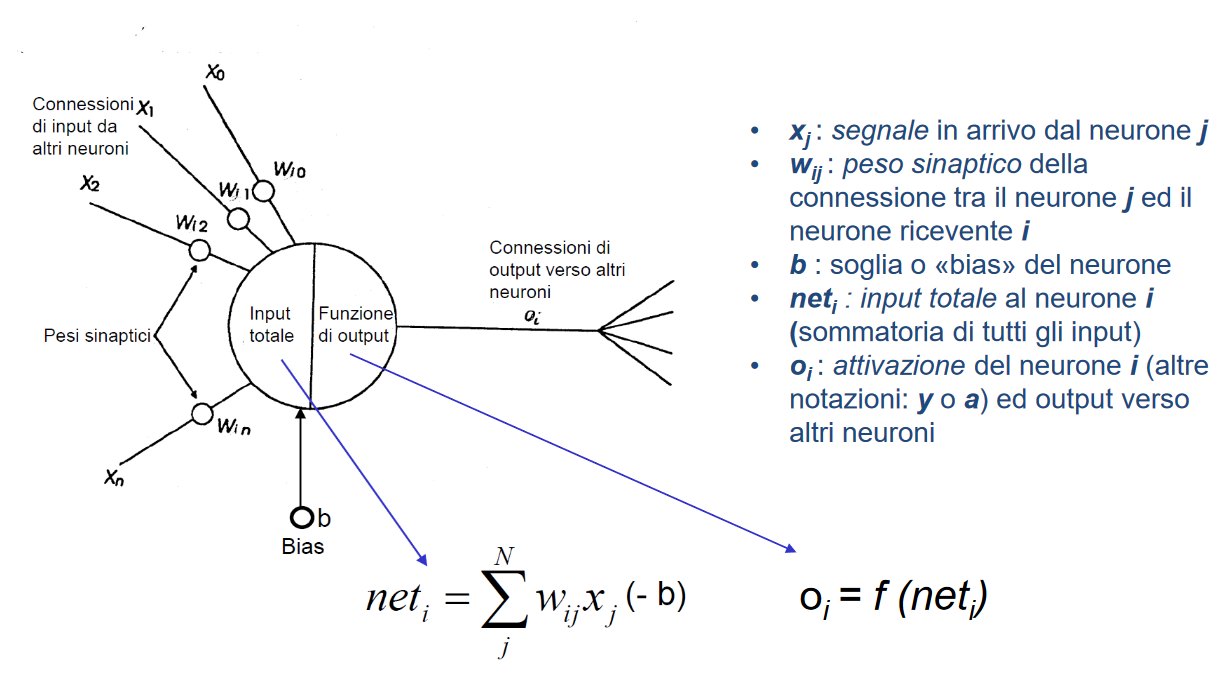
\includegraphics[width=0.9\columnwidth]{teoria/neurone.png} 
    \caption{Funzionamento del neurone}
    \label{fig:neurone}
  \end{figure}

  \begin{figure}[!h] 
    \centering 
    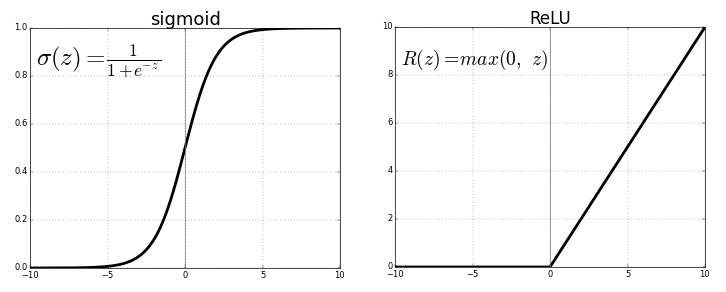
\includegraphics[width=0.8\columnwidth]{teoria/relu-sigmoid.png} 
    \caption{Funzioni di attivazione}
    \label{fig:relu-sigmoid}
  \end{figure}

\newpage

\subsubsection{Fasi di apprendimento} 
Inizialmente la rete riceve in input il vettore, i pesi e i bias vengono decisi in maniera casuale.
I dati si spostano di strato in strato fino a raggiungere quello di output (forward propagation, Fig.~\ref{fig:propagation}), successivamente la funzione di perdita misura il grado di errore e tramite la backward propagation avviene l'Aggiornamento dei pesi.
Queste fasi vengono ripetute per un numero adeguato di volte (epoche) per ridurre man mano l'errore.

\begin{figure}[!h] 
    \centering 
    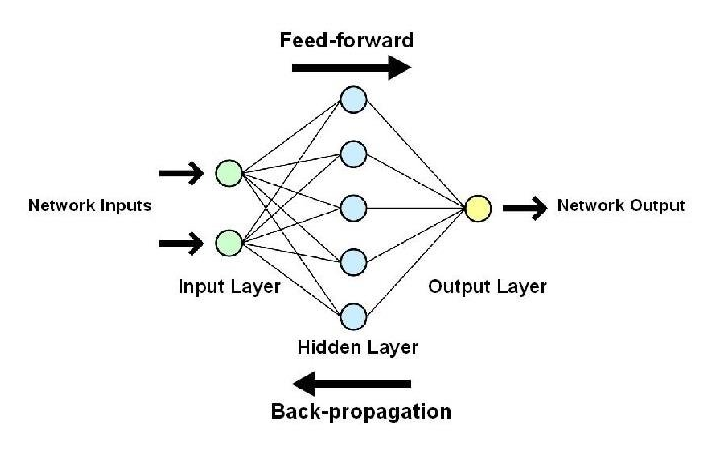
\includegraphics[width=0.6\columnwidth]{teoria/propagation.png} 
    \caption{Forward e backward propagation}
    \label{fig:propagation}
  \end{figure}

\newpage
\subsection{Classificazione}
I dati da classificare vengono inseriti all'interno della rete neurale che fornisce in output la classe di appartenenza di ciascun dato (Fig.~\ref{fig:classificazione}).

\begin{figure}[!h] 
    \centering 
    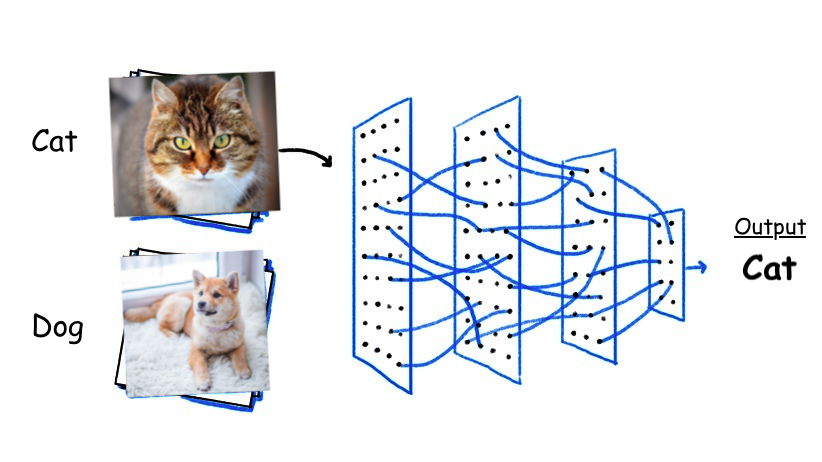
\includegraphics[width=0.6\columnwidth]{teoria/classificazione.png} 
    \caption{Classificazione dei dati}
    \label{fig:classificazione}
  \end{figure}


\section{Deep learning}
Con il termine deep learning si identificano reti neurali con un numero di strati nascosti maggiore o uguale a due (Fig.~\ref{fig:deep-learning}).

\begin{figure}[!h] 
    \centering 
    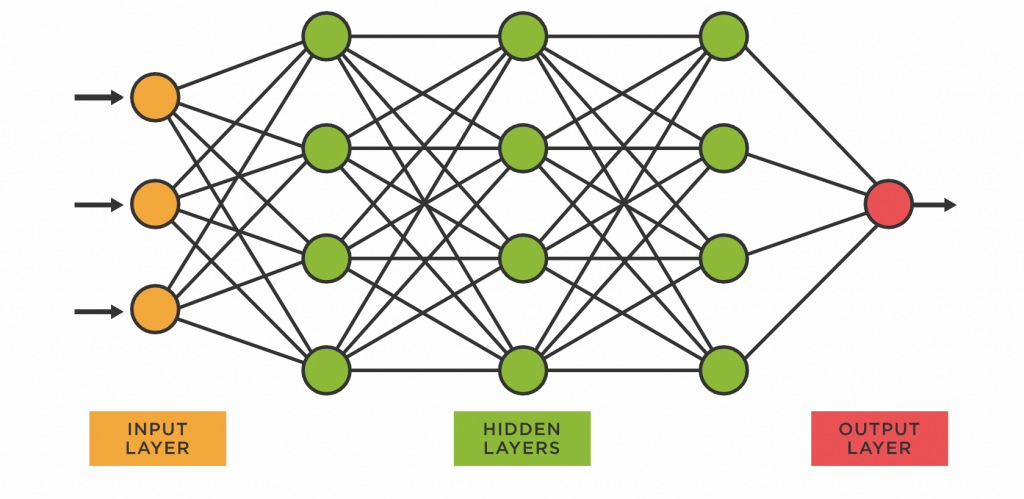
\includegraphics[width=0.8\columnwidth]{teoria/deep-learning.png} 
    \caption{Esempio di rete neurale con più strati nascosti}
    \label{fig:deep-learning}
  \end{figure}

\subsection{Convolutional neural network}
Le reti neurali convoluzionali (CNN) sono un esempio di deep learning, esse sfruttano dei layer convoluzionali per eseguire la classificazione di dati tridimensionali, come ad esempio le classiche immagini raster.
\subsubsection{Layer convoluzionali}
I layer convoluzionali hanno come scopo l'estrazione di feature dalle immagini (texture, bordi, ecc...).
Per spiegare il funzionamento di un layer convoluzionale è necessario introdurre la nozione di kernel.

Il kernel (filtro) è una matrice contenente dei pesi, che viene spostata lungo l'immagine effettuando una convoluzione in ogni posizione.
Esempio con kernel di dimensioni 3x3:

\begin{lstlisting}[language=Python, frame=none]
    [ -1,  0,  1 ]
    [ -1,  0,  1 ]
    [ -1,  0,  1 ]
\end{lstlisting}


\begin{enumerate}
    \item Posizionamento del filtro: il kernel viene inserito sulla prima zona 3x3 dell'immagine.
    \item Moltiplicazione di ogni elemento: ogni peso presente nel kernel viene moltiplicato per il valore corrispondente contenuto nella porzione di immagine.
        
    \begin{lstlisting}[language=Python, frame=none]
        PORZIONE DI IMMAGINE
        [ 10, 20, 30 ]
        [ 40, 50, 60 ]
        [ 70, 80, 90 ]

        PRODOTTO CON I PESI DEL KERNEL
        (-1 * 10) + (0 * 20) + (1 * 30) +
        (-1 * 40) + (0 * 50) + (1 * 60) +
        (-1 * 70) + (0 * 80) + (1 * 90)
            
    \end{lstlisting}
    \item Output della convoluzione: tutti i risultati delle moltiplicazioni vengono sommati tra di loro e il valore ottenuto viene posizionato nella feature map nel punto che corrisponde alla regione dell'immagine elaborata.
    \begin{lstlisting}[language=Python, frame=none]
        (-10) + (0) + (30) +
        (-40) + (0) + (60) +
        (-70) + (0) + (90) = 60
    \end{lstlisting}
    \item Riposizionamento del filtro: il kernel viene riposizionato spostandolo di uno o più pixel (stride) e il flusso si ripete fino alla copertura completa dell'immagine.
\end{enumerate}

L'otuput del layer convoluzionale è una serie di feature map ognuna corrispondente a ciascun filtro.

\begin{lstlisting}[language=Python, frame=none]
    conv_layer= Conv2D(32, (3, 3), activation='relu', padding='same')(input_img)
\end{lstlisting}

\begin{itemize}
    \item 32 rappresenta il numero di filtri.
    \item (3,3) rappresenta la dimensione dei kernel.
    \item activation='relu' indica che come funzione di attivazione verrà utilizzata relu.
    \item padding='same' consente di mantenere la dimensione dell'immagine in input anche dopo l'applicazione dei filtri
\end{itemize}


\subsubsection{Layer di pooling}
I layer di pooling servono per ridurre le dimensioni delle feature maps mantenendo le caratteristiche importanti e riducendo di conseguenza la complessità di calcolo.
\subsubsection{Funzionamento di un layer di pooling}
Esempio di Max pooling con matrici 2x2 e stride di 2 pixel

Feature map 4x4:
\begin{lstlisting}[language=Python, frame=none]
    [ 1, 3, 2, 4 ]
    [ 5, 6, 8, 7 ]
    [ 3, 2, 1, 0 ]
    [ 1, 2, 4, 3 ]
\end{lstlisting}

\begin{enumerate}
    \item Divisione della feature map in matrici 2x2:
    \begin{lstlisting}[language=Python, frame=none]
    
        [ 1, 3 ]
        [ 5, 6 ]
        
        [ 2, 4 ]
        [ 8, 7 ]
        
        [ 3, 2 ]
        [ 1, 0 ]
        
        [ 1, 2 ]
        [ 4, 3 ]

    \end{lstlisting}
    \item Calcolo del valore massimo per ogni matrice:
    
    \begin{lstlisting}[language=Python, frame=none]
        max(1, 3, 5, 6) = 6
        max(2, 4, 8, 7) = 8
        max(3, 2, 1, 0) = 3
        max(1, 2, 4, 3) = 4
    \end{lstlisting}

    \item Creazione di una nuova feature map contenente i valori massimi:
    \begin{lstlisting}[language=Python, frame=none]
        [ 6, 8 ]
        [ 3, 4 ]
    \end{lstlisting}
\end{enumerate}
L'output del layer di pooling in questo caso è una feature map ridotta da 4x4 a 2x2.

\begin{lstlisting}[language=Python, frame=none]
    MaxPooling2D((2, 2), padding='same')(x)
\end{lstlisting}

\section{Autoencoder}
L'autoencoder è un neural network in grado di comprimere il suo input e di ricostruirlo in maniera similare come output. \footcite[p.~499]{Goodfellow-et-al-2016}.
L'architettura si compone di due parti principali:
\begin{enumerate}
    \item Encoder: comprime l'input riducendolo di dimensionalità (codifica).
    \item Decoder: ricostruisce l'input inziale partendo dalla codifica fatta dall'encoder
\end{enumerate}
Il bottleneck o latent space contiene la codifica e sta nel mezzo delle due componenti; è il punto di arrivo del encoder e la partenza del decoder.

\subsection{Funzionamento}
\begin{enumerate}
    \item L'encoder riceve un input \( x \) e lo codifica creando una funzione \( z= f(x) \)
    \item Il bottleneck contiene la codifica \( z \)
    \item Il decoder cerca di decodificare \( z \) tramite la funzione \( g \) ottenendo come output \( \hat{x} = g(z) \).
\end{enumerate}

Il processo di apprendimento ha come obiettivo minimizzare la loss function che misura la differenza tra input iniziale e output ricostruito dal decoder.
\[ L(x, \hat{x}) = ||x - \hat{x}||^2 \]
Nell'esempio viene utilizzata la MSE (Mean Squared Error).

Ai fini del progetto la parte interessante dell'autoencoder è proprio l'encoder perchè comprime l'immagine in input lasciando un set di features nel bottleneck; che possono essere utilizzate successivamente per il clustering.







